\documentclass[17pt, a0paper, landscape]{tikzposter} 
\tikzposterlatexaffectionproofoff 

\usepackage{amsmath,amssymb}
\usepackage[shortlabels]{enumitem}
\usepackage{graphicx}
\usepackage{parskip}
\usepackage[unicode]{hyperref}
\usepackage{pgfplots}
\pgfplotsset{compat=1.15}
\usepackage{mathrsfs}
\usetikzlibrary{arrows, calc, intersections, positioning}

% --- تنظیم ابعاد صفحه ---
\geometry{paperwidth=118.9cm, paperheight=119cm, margin=1cm}

% تنظیم رنگ‌ها
\usepackage{xcolor}
\usepackage[normalem]{ulem}
\useunder{\uline}{\ulined}{}%
\DeclareUrlCommand{\bulurl}{\def\UrlFont{\ttfamily\color{blue}\ulined}}

% --- تنظیمات فارسی (باید آخرین بسته باشد) ---
\usepackage{xepersian}
\settextfont{XB Niloofar} 
\setlatintextfont{Liberation Serif}
\setdigitfont{Yas}

% ============================================================
% راه حل قطعی برای وسط‌چین کردن عناوین بلوک‌ها در زی‌پرشین
% ============================================================
\makeatletter
% ذخیره دستور اصلی بلوک
\let\oldblock\block
% بازتعریف دستور بلوک
\renewcommand{\block}[2]{%
    % محاسبه عرض بلوک (تقریبی بر اساس عرض ستون 0.14)
    % ما متن عنوان را در یک جعبه وسط‌چین (center) قرار می‌دهیم
    \oldblock{\begin{center}\parbox{14cm}{\centering #1}\end{center}}{#2}%
}
\makeatother
% ============================================================

% تعریف رنگ‌های پوستر
\definecolorpalette{PurpleGrayBlue}{
    \definecolor{colorOne}{HTML}{D40279}
    \definecolor{colorTwo}{HTML}{7F8897}
    \definecolor{colorThree}{HTML}{006C9E}
}

% تنظیمات عنوان اصلی
\settitle{\centering \@title}
\title{\textcolor[HTML]{D40279}{\textbf{\Huge{آمادگی برای آزمون ریاضی: هندسه مسطحه}}}}

\makeatletter
\newcommand\insertlogoi[2][]{\def\@insertlogoi{\includegraphics[#1]{#2}}}
\newcommand\insertlogoii[2][]{\def\@insertlogoii{\includegraphics[#1]{#2}}}
\newlength\LogoSep
\setlength\LogoSep{0pt}

\insertlogoi[width=10cm]{figures/logo.pdf} 
\insertlogoii[width=5cm]{example-image-b}

\renewcommand\maketitle[1][]{  
    \normalsize
    \setkeys{title}{#1}
    \node[transparent,inner sep=\TP@titleinnersep, line width=\TP@titlelinewidth, anchor=north, minimum width=\TP@visibletextwidth-2\TP@titleinnersep]
        (TP@title) at ($(0, 0.5\textheight-\TP@titletotopverticalspace)$) {\parbox{\TP@titlewidth-2\TP@titleinnersep}{\TP@maketitle}};
    \draw let \p1 = ($(TP@title.north)-(TP@title.south)$) in node {
        \setlength{\TP@titleheight}{\y1}
        \setlength{\titleheight}{\y1}
        \global\TP@titleheight=\TP@titleheight
        \global\titleheight=\titleheight
    };

    \setlength{\titleposleft}{-0.5\titlewidth}
    \setlength{\titleposright}{\titleposleft+\titlewidth}
    \setlength{\titlepostop}{0.5\textheight-\TP@titletotopverticalspace}
    \setlength{\titleposbottom}{\titlepostop-\titleheight}

    \TP@titlestyle

    \node[inner sep=\TP@titleinnersep, line width=\TP@titlelinewidth, anchor=north, minimum width=\TP@visibletextwidth-2\TP@titleinnersep]
        at (0,0.5\textheight-\TP@titletotopverticalspace)
        (title)
        {\parbox{\TP@titlewidth-2\TP@titleinnersep}{\begin{center}\TP@maketitle\end{center}}}; 

    \node[inner sep=400pt,anchor=west] 
      at ([xshift=-\LogoSep]title.west)
      {\@insertlogoi};

    \node[inner sep=400pt,anchor=east] 
      at ([xshift=\LogoSep]title.east)
      {\Huge\bulurl{https://plucik.ru/}};

    \normalsize
    \setlength{\TP@blocktop}{\titleposbottom-\TP@titletoblockverticalspace}
}
\makeatother

\usetheme{Simple}
\colorlet{titlebgcolor}{white}
\usetitlestyle{Default}
\useblockstyle{TornOut}

% علامت توازی
\newcommand{\parallelsum}{\mathbin{\|}}

\begin{document}

\begin{RTL}

% تعریف رنگ‌ها برای تصاویر
\definecolor{atfczz}{rgb}{0,0.6,0}
\definecolor{fruycc}{rgb}{0.8313725490196079,0.00784313725490196,0.4745098039215686}
\definecolor{qqwuqq}{rgb}{0,0.6,0}
\definecolor{ududff}{rgb}{0.8313725490196079,0.00784313725490196,0.4745098039215686}
\definecolor{qqqqff}{rgb}{0.8313725490196079,0.00784313725490196,0.4745098039215686}
\definecolor{atfcqq}{rgb}{0,0.6,0}
\definecolor{xdxdff}{rgb}{0.8313725490196079,0.00784313725490196,0.4745098039215686}
\definecolor{duqsxz}{rgb}{0.8313725490196079,0.00784313725490196,0.4745098039215686}

\maketitle

\begin{columns}
% ستون اول (راست)
\column{0.14}
\block{قضیه تالس}
{
$$l_1 \ \parallelsum \ l_2 \ \parallelsum \ l_3 \iff \frac {a} {a'} = \frac {b} {b'} = \frac {c} {c'}$$
\begin{center}
\begin{latin}
\input{figures/thales_plain.tex}
\end{latin}
\end{center}
}
\block{نقطه برخورد میانه‌ها}
{
$$\frac {CO} {OM} = \frac {AO} {OD} = \frac {BO} {OE} = \frac {2} {1}$$
\begin{center}
\begin{latin}
\input{figures/median_plain.tex}
\end{latin}
\end{center}
}
\block{ویژگی خاص ذوزنقه}
{
\begin{center}
$F, M$ وسطِ قاعده‌های ذوزنقه $ABCD$\\
$\Rightarrow$ نقاط $E, F, M$ هم‌خط هستند \\
\begin{latin}
\input{figures/trapezoid_plain.tex}
\end{latin}
\end{center}
}
\block{قضیه فیثاغورس}
{
$$\Delta ABC \text{ قائم‌الزاویه } \iff a^2 + b^2 = c^2$$
\begin{center}
\begin{latin}
\input{figures/pythagoras_plain.tex}
\end{latin}
\end{center}
}
\block{ارتفاع در مثلث قائم‌الزاویه}
{
$$h^2 = x \cdot y$$
\begin{center}
\begin{latin}
\input{figures/h_right_plain.tex}
\end{latin}
\end{center}
}

% ستون دوم
\column{0.14}
\block{قضیه سینوس‌ها}
{
$$\frac {a} {\sin{\alpha}} = \frac {b} {\sin{\beta}} = \frac {c} {\sin{\gamma}} = 2R$$
\begin{center}
\begin{latin}
\input{figures/sin_plain.tex}
\end{latin}
\end{center}
}
\block{قضیه کسینوس‌ها}
{
$$c^2 = a^2 + b^2 - 2ab\cdot\cos{\gamma}$$
\begin{center}
\begin{latin}
\input{figures/cos_plain.tex}
\end{latin}
\end{center}
}
\block{قضیه منلائوس}
{
$$\frac {AN} {NB} \cdot \frac {BM} {MC} \cdot \frac {CK} {KA} = 1$$
\begin{center}
\begin{latin}
\input{figures/menelai_plain.tex}
\end{latin}
\end{center}
}
\block{قضیه سوا (Ceva)}
{
$$\frac {AM} {MB} \cdot \frac {BN} {NC} \cdot \frac {CK} {KA} = 1$$
\begin{center}
\begin{latin}
\input{figures/cheva_plain.tex}
\end{latin}
\end{center}
}
\block{قضیه وان اوبل}
{
$$\frac {BO} {OK} = \frac {BN} {NC} + \frac {BM} {MA}$$
\begin{center}
\begin{latin}
\input{figures/van-obel_plain.tex}
\end{latin}
\end{center}
}

% ستون سوم
\column{0.14}
\block{قضیه نیمساز}
{
$$\frac {a} {b} = \frac {x} {y}$$
\begin{center}
\begin{latin}
\input{figures/bisector_plain.tex}
\end{latin}
\end{center}
}
\block{مساحت مثلث}
{
$$S_\Delta = \frac 1 2 \cdot ah = \frac 1 2 \cdot ab \cdot \sin{\alpha}$$
\begin{center}
\begin{latin}
\begin{tikzpicture}[line cap=round,line join=round,>=triangle 45,x=1cm,y=1cm, every node/.style={scale=2}]
\draw[line width=2pt,color=atfczz,fill=atfczz,fill opacity=0.1] (5.569728971410907,0) -- (5.569728971410907,0.5697289714109068) -- (5,0.5697289714109067) -- (5,0) -- cycle; 
\draw [shift={(13,0)},line width=2pt,color=qqwuqq,fill=qqwuqq,fill opacity=0.10000000149011612] (0,0) -- (138.81407483429035:1.2085776573692664) arc (138.81407483429035:180:1.2085776573692664) -- cycle;
\draw [line width=2pt] (0,0)-- (5,7);
\draw [line width=2pt] (5,7)-- (13,0);
\draw [line width=2pt] (5,7)-- (5,0);
\draw [line width=2pt] (0,0)-- (13,0);
\begin{scriptsize}
\draw [fill=ududff] (0,0) circle (2.5pt);
\draw [fill=qqqqff] (13,0) circle (2.5pt);
\draw [fill=qqqqff] (5,7) circle (2.5pt);
\draw [fill=qqqqff] (5,0) circle (2.5pt);
\draw[color=black] (9.128371227823514,4.404974508154897) node {$b$};
\draw[color=black] (4.435061325039529,3.4179694213033307) node {$h$};
\draw[color=black] (6.570215186391899,-0.4) node {$a$};
\draw[color=qqwuqq] (11,0.7) node {$\alpha$};
\end{scriptsize}
\end{tikzpicture}
\end{latin}
\end{center}
}
\block{فرمول هرون}
{
$$p = \frac {a + b + c} {2},$$
$$S_\Delta = \sqrt{p(p-a)(p-b)(p-c)}$$
\vspace{0.5cm}
\begin{center}
\begin{latin}
\input{figures/geron_plain.tex}
\end{latin}
\end{center}
}
\block{مساحت ذوزنقه}
{
$$S_{ABCD} = \frac {AD + BC} {2}\cdot h$$
\begin{center}
\begin{latin}
\input{figures/trapezoid_area_plain.tex}
\end{latin}
\end{center}
}
\block{مساحت چهارضلعی}
{
$$S_{ABCD} = \frac 1 2 \cdot AC \cdot BD \cdot \sin{\alpha}$$
\begin{center}
\begin{latin}
\input{figures/4p_area_plain.tex}
\end{latin}
\end{center}
}

% ستون چهارم
\column{0.14}
\block{نسبت مساحت‌ها}
{
(با زاویه مشترک)
$$\frac {S_{\Delta ABC}} {S_{\Delta ADE}} = \frac {AB} {AD} \cdot \frac {AC} {AE}$$
\begin{center}
\begin{latin}
\input{figures/area_frac_plain.tex}
\end{latin}
\end{center}
}
\block{زوایای محاطی}
{
$$\angle{AEB} = \angle{ADB} = \frac 1 2 \smallsmile{AB}$$
\begin{center}
\begin{latin}
\input{figures/duga_plain.tex}
\end{latin}
\end{center}
}
\block{زاویه مماس و وتر}
{
$$\angle{ABC} = \angle{ADB} = \frac 1 2 \smallsmile{AB}$$
\begin{center}
\begin{latin}
\input{figures/kas_angle_plain.tex}
\end{latin}
\end{center}
}
\block{زاویه بین دو وتر}
{
$$\angle{AKB} = \angle{EKD} = \frac {\smallsmile{AB} \ + \smallsmile{ED}} {2}$$
\begin{center}
\begin{latin}
\input{figures/chord_angle_plain.tex}
\end{latin}
\end{center}
}
\block{زاویه بین دو قاطع}
{
$$\angle{BAC} = \frac {\smallsmile {DE} \ - \smallsmile{BC}} {2}$$
\begin{center}
\begin{latin}
\input{figures/sec_angle_plain.tex}
\end{latin}
\end{center}
}

% ستون پنجم
\column{0.14}
\block{زوایا در خطوط موازی}
{
$$k \ \parallelsum \ l \iff \alpha = \beta = \gamma$$
\begin{center}
\begin{latin}
\input{figures/parallel_plain.tex}
\end{latin}
\end{center}
}
\block{دو مماس از یک نقطه}
{
$$AB = AC$$
\begin{center}
\begin{latin}
\input{figures/2kas_plain.tex}
\end{latin}
\end{center}
}
\block{رابطه مماس و قاطع}
{
$$\Delta ABC \sim \Delta ADB, \quad AB^2 = AC \cdot AD$$
\begin{center}
\begin{latin}
\input{figures/kas_plain.tex}
\end{latin}
\end{center}
}
\block{وترهای متقاطع}
{
$$\Delta AKB \sim \Delta EKD, \quad AK \cdot KD = BK \cdot KE$$
\vspace{0.5cm}
\begin{center}
\begin{latin}
\input{figures/chord_plain.tex}
\end{latin}
\end{center}
}
\block{رابطه دو قاطع}
{
$$\Delta ABC \sim \Delta ADE, \quad AB \cdot AD = AC \cdot AE$$
\begin{center}
\begin{latin}
\input{figures/sec_plain.tex}
\end{latin}
\end{center}
}

% ستون ششم
\column{0.14}
\block{دایره محاطی مثلث}
{
\begin{center}
مرکز: محل برخورد نیمسازهای داخلی \\
\vspace{0.5cm}
\begin{latin}
\input{figures/cvt_plain.tex}
\end{latin}
\end{center}
}
\block{دایره محیطی مثلث}
{
\begin{center}
مرکز: محل برخورد عمودمنصف‌ها \\
\vspace{0.5cm}
\begin{latin}
\input{figures/cot_plain.tex}
\end{latin}
\end{center}
}
\block{محیطی (مثلث قائم‌الزاویه)}
{
\begin{center}
$\Delta ABC$ قائم‌الزاویه $\iff AC$ قطر است،\\
AO = OC = OB = R\\
\vspace{0.5cm}
\begin{latin}
\input{figures/ort_plain.tex}
\end{latin}
\end{center}
}
\block{چهارضلعی محاطی}
{
\begin{center}
$ABCD$ محاطی $\iff \alpha + \beta = 180^\circ$\\
\vspace{0.5cm}
\begin{latin}
\begin{tikzpicture}[line cap=round,line join=round,>=triangle 45,x=1cm,y=1cm, every node/.style={scale=2}]
\draw [shift={(1.2391441753682169,5.551647976431845)},line width=2pt,color=atfczz,fill=atfczz,fill opacity=0.1] (0,0) -- (-77.90850664840158:0.8212560386473431) arc (-77.90850664840158:14.02165447024648:0.8212560386473431) -- cycle;
\draw [shift={(7.927735410246219,1.9157466518178983)},line width=2pt,color=duqsxz,fill=duqsxz,fill opacity=0.1] (0,0) -- (91.11584740696172:0.8212560386473431) arc (91.11584740696172:179.18568628831366:0.8212560386473431) -- cycle;
\draw [line width=2pt] (5,4.5) circle (3.905124837953328cm);
\draw [line width=2pt] (1.2391441753682169,5.551647976431845)-- (7.82488249596053,7.196300963174513);
\draw [line width=2pt] (7.82488249596053,7.196300963174513)-- (7.927735410246219,1.9157466518178983);
\draw [line width=2pt] (7.927735410246219,1.9157466518178983)-- (2,2);
\draw [line width=2pt] (2,2)-- (1.2391441753682169,5.551647976431845);
\begin{scriptsize}
\draw [fill=qqqqff] (2,2) circle (2.5pt);
\draw[color=qqqqff] (1.6514837819185615,1.8165401426270997) node {$A$};
\draw [fill=xdxdff] (7.927735410246219,1.9157466518178983) circle (2.5pt);
\draw[color=xdxdff] (8.256728778467908,1.769611226132966) node {$D$};
\draw [fill=xdxdff] (1.2391441753682169,5.551647976431845) circle (2.5pt);
\draw[color=xdxdff] (0.7481021394064841,5.711640211640212) node {$B$};
\draw [fill=xdxdff] (7.82488249596053,7.196300963174513) circle (2.5pt);
\draw[color=xdxdff] (8.104209799861973,7.506671267540834) node {$C$};
\draw[color=atfczz] (2.5,4.9) node {$\alpha$};
\draw[color=duqsxz] (7.1,2.7) node {$\beta$};
\end{scriptsize}
\end{tikzpicture}
\end{latin}
\end{center}
}
\block{چهارضلعی محیطی}
{
\begin{center}
$ABCD$ محیطی $\iff AB + CD = BC + AD$\\
\vspace{0.5cm}
\begin{latin}
\input{figures/o4_plain.tex}
\end{latin}
\end{center}
}

% ستون هفتم (موارد اضافه شده)
\column{0.14}

\block{قضیه استوارت}
{
$$b^2m + c^2n = a(d^2 + mn)$$
\begin{center}
\begin{latin} 
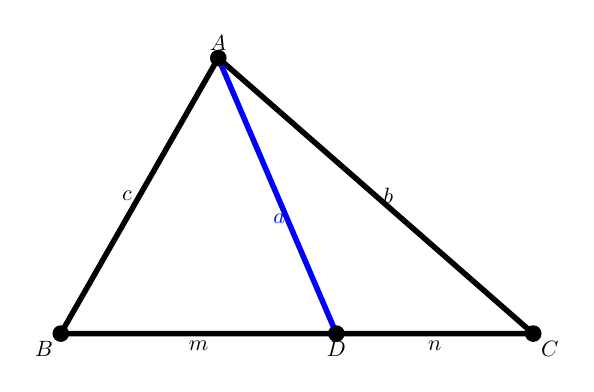
\begin{tikzpicture}[line cap=round,line join=round,>=triangle 45,x=1cm,y=1cm, every node/.style={scale=0.8}]
% Triangle Nodes
\coordinate (B) at (0,0);
\coordinate (C) at (6,0);
\coordinate (A) at (2,3.5);
\coordinate (D) at (3.5,0);

% Draw
\draw [line width=2pt] (A) -- (B) -- (C) -- cycle;
\draw [line width=2pt, color=blue] (A) -- (D);

% Labels
\node [above] at (A) {$A$};
\node [below left] at (B) {$B$};
\node [below right] at (C) {$C$};
\node [below] at (D) {$D$};

% Segment Labels
\node [left] at (1,1.75) {$c$};
\node [right] at (4,1.75) {$b$};
\node [below] at (1.75,0) {$m$};
\node [below] at (4.75,0) {$n$};
\node [right, color=blue] at (2.6,1.5) {$d$};

\foreach \point in {A,B,C,D} \fill [color=black] (\point) circle (3pt);
\end{tikzpicture}
\end{latin}
\end{center}
}

\block{قضیه بطلمیوس}
{
$$AC \cdot BD = AB \cdot CD + BC \cdot DA$$
\begin{center}
\begin{latin}
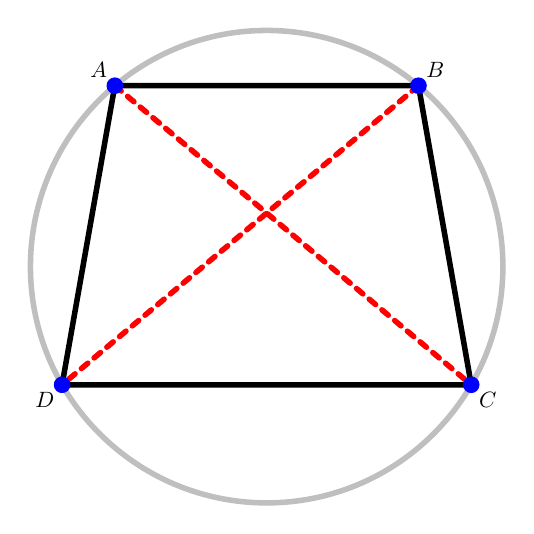
\begin{tikzpicture}[line cap=round,line join=round,>=triangle 45,x=1cm,y=1cm, every node/.style={scale=0.8}]
% Circle
\draw [line width=2pt, color=gray!50] (0,0) circle (3cm);

% Coordinates on circle
\coordinate (A) at (130:3);
\coordinate (B) at (50:3);
\coordinate (C) at (-30:3);
\coordinate (D) at (-150:3);

% Draw Quadrilateral
\draw [line width=2pt] (A) -- (B) -- (C) -- (D) -- cycle;

% Draw Diagonals
\draw [line width=2pt, dashed, color=red] (A) -- (C);
\draw [line width=2pt, dashed, color=red] (B) -- (D);

% Labels
\node [above left] at (A) {$A$};
\node [above right] at (B) {$B$};
\node [below right] at (C) {$C$};
\node [below left] at (D) {$D$};

% Points
\foreach \point in {A,B,C,D}
\fill [color=blue] (\point) circle (3pt);
\end{tikzpicture}
\end{latin}
\end{center}
}

\block{طول میانه}
{
$$m_a^2 = \frac{2b^2 + 2c^2 - a^2}{4}$$
\begin{center}
\begin{latin}
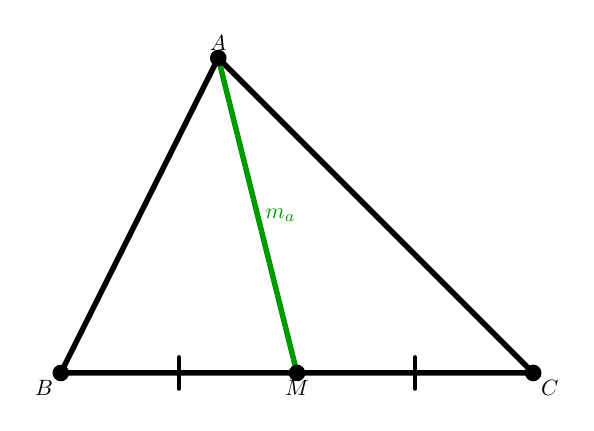
\begin{tikzpicture}[line cap=round,line join=round,>=triangle 45,x=1cm,y=1cm, every node/.style={scale=0.8}]
% Triangle
\coordinate (B) at (0,0);
\coordinate (C) at (6,0);
\coordinate (A) at (2,4);
\coordinate (M) at (3,0); % Midpoint

% Draw
\draw [line width=2pt] (A) -- (B) -- (C) -- cycle;
\draw [line width=2pt, color=green!60!black] (A) -- (M);

% Tick marks for midpoint
\draw [line width=1.5pt] (1.5, -0.2) -- (1.5, 0.2);
\draw [line width=1.5pt] (4.5, -0.2) -- (4.5, 0.2);

% Labels
\node [above] at (A) {$A$};
\node [below left] at (B) {$B$};
\node [below right] at (C) {$C$};
\node [below] at (M) {$M$};
\node [right, color=green!60!black] at (2.5, 2) {$m_a$};

% Points
\foreach \point in {A,B,C,M}
\fill [color=black] (\point) circle (3pt);
\end{tikzpicture}
\end{latin}
\end{center}
}

\block{طول نیمساز}
{
$$l_a^2 = bc - mn$$
\begin{center}
\begin{latin}
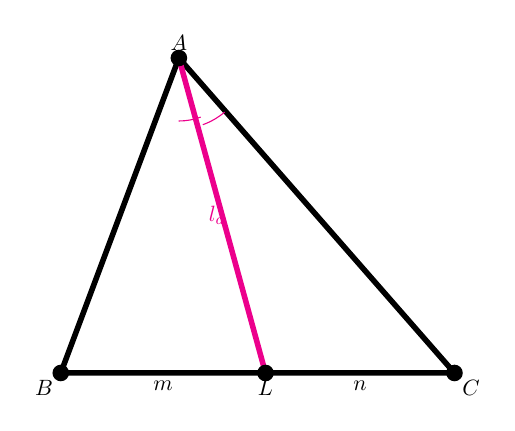
\begin{tikzpicture}[line cap=round,line join=round,>=triangle 45,x=1cm,y=1cm, every node/.style={scale=0.8}]
% Triangle
\coordinate (B) at (0,0);
\coordinate (C) at (5,0);
\coordinate (A) at (1.5,4);
\coordinate (L) at (2.6,0); % Approximate foot of bisector

% Draw
\draw [line width=2pt] (A) -- (B) -- (C) -- cycle;
\draw [line width=2pt, color=magenta] (A) -- (L);

% Angle Marks
\draw [shift={(1.5,4)}, color=magenta] (-70:0.8) arc (-70:-90:0.8);
\draw [shift={(1.5,4)}, color=magenta] (-50:0.9) arc (-50:-70:0.9);

% Labels
\node [above] at (A) {$A$};
\node [below left] at (B) {$B$};
\node [below right] at (C) {$C$};
\node [below] at (L) {$L$};
\node [left, color=magenta] at (2.2, 2) {$l_a$};
\node [below] at (1.3,0) {$m$};
\node [below] at (3.8,0) {$n$};

% Points
\foreach \point in {A,B,C,L}
\fill [color=black] (\point) circle (3pt);
\end{tikzpicture}
\end{latin}
\end{center}
}

\block{خط اویلر}
{
\begin{center}
$H, G, O$ هم‌خط هستند و $HG = 2GO$\\
\vspace{0.5cm}
\begin{latin}
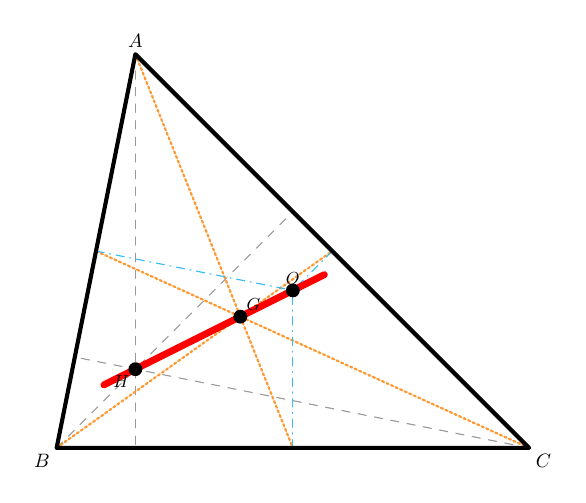
\begin{tikzpicture}[line cap=round,line join=round,>=triangle 45,x=1cm,y=1cm, every node/.style={scale=0.7}]
% مختصات رئوس
\coordinate (A) at (-1, 3);
\coordinate (B) at (-2, -2);
\coordinate (C) at (4, -2);

% --- محاسبه نقاط اصلی ---
% 1. مرکز ارتفاعی (H)
\coordinate (H) at (-1, -1);
% 2. مرکز ثقل (G)
\coordinate (G) at (0.333, -0.333);
% 3. مرکز دایره محیطی (O)
\coordinate (O) at (1, 0);

% --- محاسبه نقاط کمکی برای رسم خطوط ---
% وسط اضلاع (برای میانه و عمودمنصف)
\coordinate (M_BC) at ($(B)!0.5!(C)$);
\coordinate (M_AC) at ($(A)!0.5!(C)$);
\coordinate (M_AB) at ($(A)!0.5!(B)$);

% پای ارتفاع‌ها (برای ارتفاع)
\coordinate (H_A) at ($(B)!(A)!(C)$);
\coordinate (H_B) at ($(A)!(B)!(C)$);
\coordinate (H_C) at ($(A)!(C)!(B)$);


% --- رسم خطوط سازنده (کمرنگ) ---

% 1. رسم ارتفاع‌ها (Altitudes) -> سازنده نقطه H
% استایل: خط‌چین خاکستری
\draw [dashed, thin, gray!80] (A) -- (H_A);
\draw [dashed, thin, gray!80] (B) -- (H_B);
\draw [dashed, thin, gray!80] (C) -- (H_C);

% 2. رسم میانه‌ها (Medians) -> سازنده نقطه G
% استایل: نقطه‌چین نارنجی متراکم
\draw [densely dotted, thick, orange!80] (A) -- (M_BC);
\draw [densely dotted, thick, orange!80] (B) -- (M_AC);
\draw [densely dotted, thick, orange!80] (C) -- (M_AB);

% 3. رسم عمودمنصف‌ها (Perpendicular Bisectors) -> سازنده نقطه O
% استایل: خط‌چین آبی کم‌رنگ (از وسط ضلع به سمت O وصل می‌کنیم)
\draw [dashdotted, thin, cyan!80] (M_BC) -- (O);
\draw [dashdotted, thin, cyan!80] (M_AC) -- (O);
\draw [dashdotted, thin, cyan!80] (M_AB) -- (O);


% --- رسم اجزای اصلی ---
% رسم مثلث اصلی
\draw [line width=1.5pt] (A) -- (B) -- (C) -- cycle;

% رسم خط اویلر (قرمز ضخیم)
\draw [line width=2.5pt, color=red] (-1.4, -1.2) -- (1.4, 0.2);

% --- رسم نقاط و نام‌گذاری ---
\fill [color=black] (H) circle (2.5pt) node[below left, scale=0.9] {$H$};
\fill [color=black] (G) circle (2.5pt) node[above right, scale=0.9] {$G$};
\fill [color=black] (O) circle (2.5pt) node[above, scale=0.9] {$O$};

\node at (A) [above] {$A$};
\node at (B) [below left] {$B$};
\node at (C) [below right] {$C$};

\end{tikzpicture}
\end{latin}
\end{center}
}

\block{خط سیمسون}
{
\begin{center}
پای عمودهای وارد بر اضلاع از نقطه‌ای روی دایره محیطی، هم‌خط هستند.\\
\vspace{0.5cm}
\begin{latin}
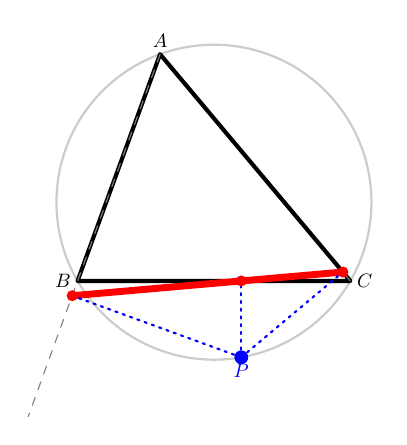
\begin{tikzpicture}[line cap=round,line join=round,>=triangle 45,x=1cm,y=1cm, every node/.style={scale=0.7}]
\coordinate (O) at (0,0);
\draw [gray!40, thick] (O) circle (2cm);

% رئوس
\coordinate (A) at (110:2cm);
\coordinate (B) at (210:2cm);
\coordinate (C) at (-30:2cm);
\coordinate (P) at (-80:2cm);

% رسم مثلث
\draw [line width=1.5pt] (A) -- (B) -- (C) -- cycle;

% محاسبه پای عمودها
\coordinate (F_BC) at ($(B)!(P)!(C)$);
\coordinate (F_AC) at ($(A)!(P)!(C)$);
\coordinate (F_AB) at ($(A)!(P)!(B)$);

% رسم خط سیمسون (قرمز ضخیم)
\draw [line width=2.5pt, color=red] (F_AB) -- (F_AC) -- (F_BC);

% خط‌چین‌های راهنما
\draw [dotted, blue, thick] (P) -- (F_BC);
\draw [dotted, blue, thick] (P) -- (F_AC);
\draw [dotted, blue, thick] (P) -- (F_AB);

% امتداد اضلاع (برای اینکه پای عمود روی هوا نباشد)
\draw [dashed, gray] (A) -- ($(A)!1.5!(F_AB)$);
\draw [dashed, gray] (C) -- ($(C)!1.2!(F_AC)$);

% نقاط
\fill [red] (F_BC) circle (2pt);
\fill [red] (F_AC) circle (2pt);
\fill [red] (F_AB) circle (2pt);
\fill [blue] (P) circle (2.5pt) node[below] {$P$};

\node at (A) [above] {$A$};
\node at (B) [left] {$B$};
\node at (C) [right] {$C$};

\end{tikzpicture}
\end{latin}
\end{center}
}

\end{columns}
\end{RTL}
\end{document}